



\begin{section}{Ejercicio 6}
Realizar un grafico del ECM de cada estimador con n = 15 y 0,5 < b < 2. ¿Que observa?
¿Que estimador elige?

\begin{subsection}{Implementacion}


Se utiliza el siguiente codigo para generar los vectores.
\begin{verbatim}
steps = 150;
b0 = 0.5;
bn = 1.5;
step = (bn-b0)/steps;
b = b0;
Bs = double();
n = 15;

momSims = double();
medSims = double();
mvSims = double();

for(i in 1:steps){
	momSims[i] <- simulacion_mom(b,n);
	medSims[i] <- simulacion_med(b,n);
	mvSims[i] <- simulacion_mv(b,n);
	b = b+step;
}
\end{verbatim}
Los graficos obtenidos son los siguientes.

~\\
~\\

Error cuadratico medio de $B_{mom}$
\begin{figure}[H]
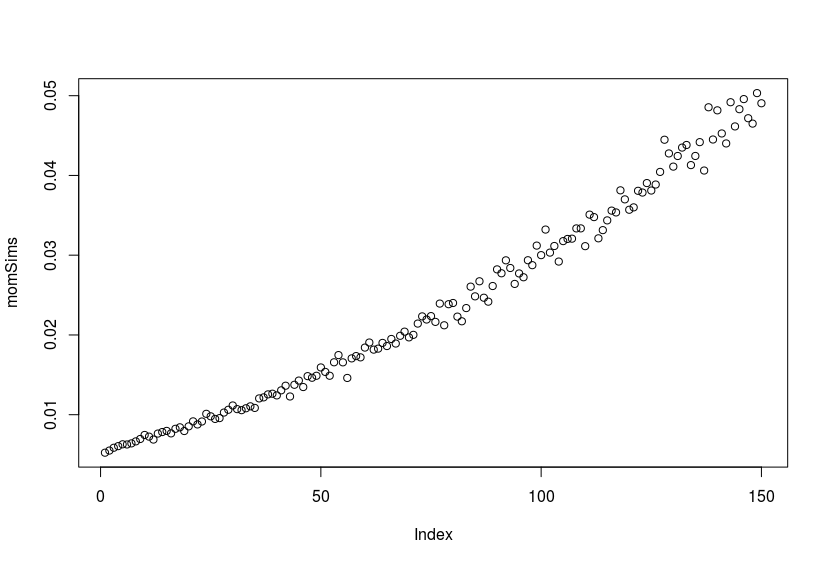
\includegraphics[scale=0.65]{plots/momSims.png}
\centering
\end{figure}
~\\
~\\

Error cuadratico medio de $B_{med}$
\begin{figure}[H]
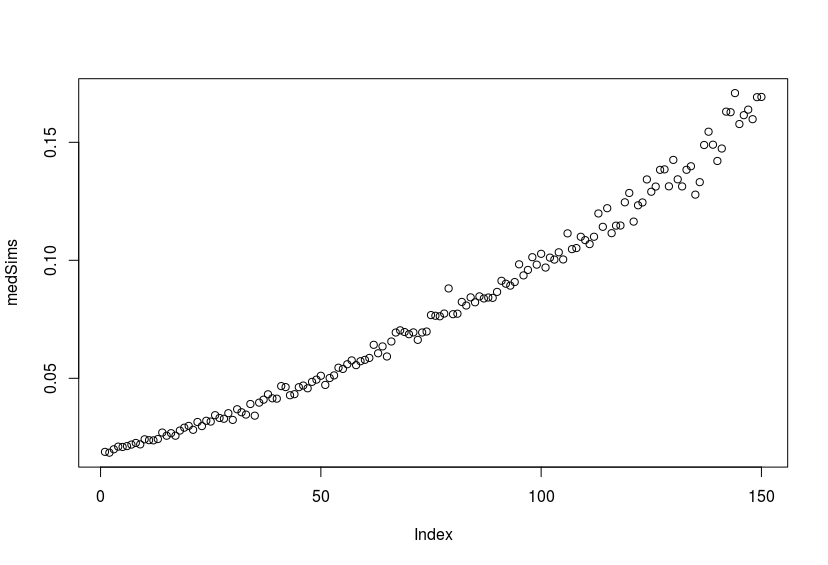
\includegraphics[scale=0.65]{plots/medSims.png}
\centering
\end{figure}
~\\
~\\

Error cuadratico medio de $B_{mv}$
\begin{figure}[H]
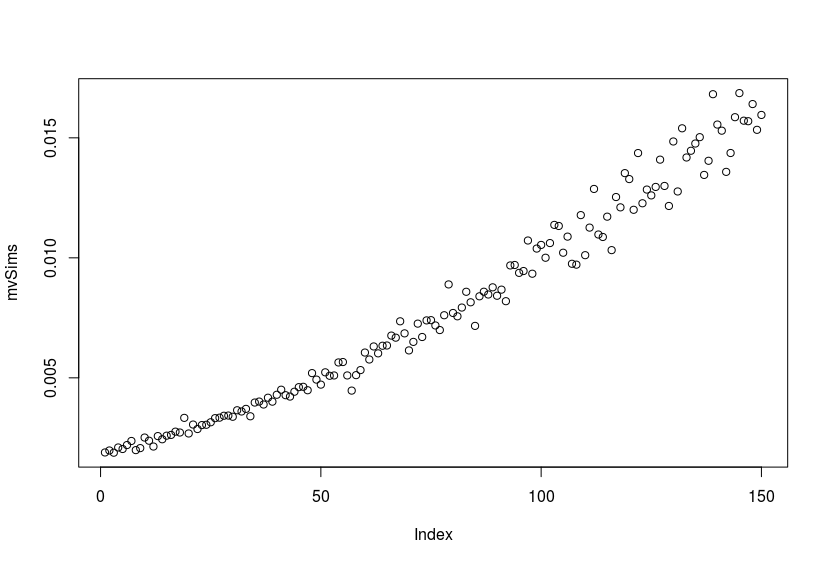
\includegraphics[scale=0.65]{plots/mvSims.png}
\centering
\end{figure}
~\\
~\\
Como puede eobservarse la magnitud del error es menor en el estimador de maxima verosimilitud, $B_{mv}$, que en los otros dos. Siendo el mestimador $B_{med}$ el que peor aproxima. Notar que si bien los datos en el grafico de $B_{mv}$ se ven mas dispersos, esto es asi gracias a que la escala vertical es menor, dado que el error lo es.
Respondiendo a la pregunta del enunciado, bajo esta medida, el estimador $B_{mv}$ funciona mejor que los otros dos, por lo cual elegiria ese.

\end{subsection}
\end{section}